% Auto-generated by scripts/plot_msshape.py — do not edit by hand.
% Preamble: \usepackage{pgfplots} \pgfplotsset{compat=1.18}
\colorlet{ourscolor}{red!70!black}
\colorlet{basecolor}{blue!50!black}
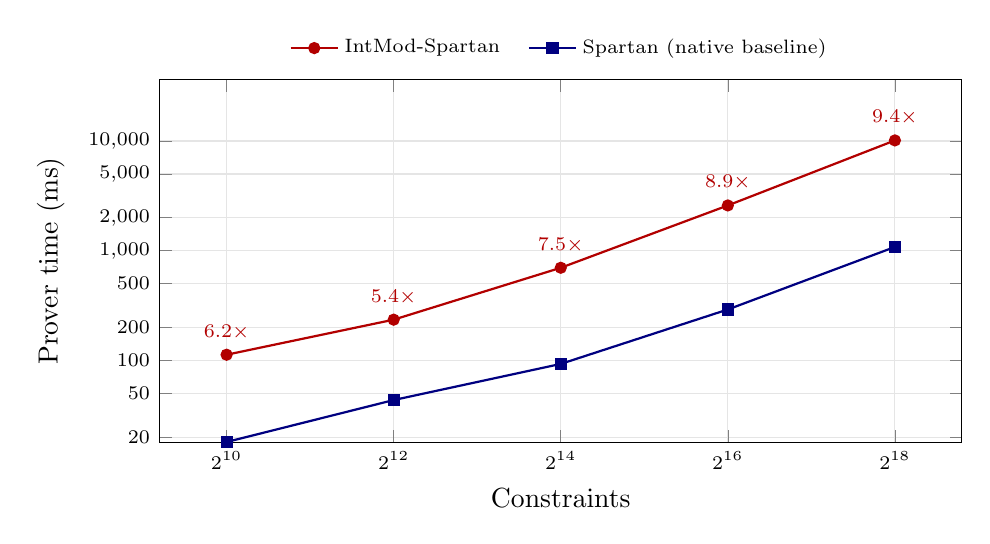
\begin{tikzpicture}
  \begin{axis}[
    scale only axis, width=0.84\linewidth, height=4.6cm,
    yticklabel style={font=\scriptsize, text width=2.4em, align=right},
    xticklabel style={font=\scriptsize},
    ymode=log,
    ytick={20,50,100,200,500,1000,2000,5000,10000}, log ticks with fixed point,
    xtick={10,12,14,16,18}, xticklabels={$2^{10}$,$2^{12}$,$2^{14}$,$2^{16}$,$2^{18}$},
    xlabel={Constraints}, ylabel={Prover time (ms)},
    grid=both, grid style={gray!20},
    % legend above the axes so it never occludes either series
    legend style={at={(0.5,1.03)}, anchor=south, legend columns=-1,
      font=\scriptsize, draw=none, /tikz/every even column/.append style={column sep=8pt}},
    enlarge y limits={upper, value=0.2},
    error bars/y dir=both, error bars/y explicit,
  ]
    \addplot[ourscolor, thick, mark=*, mark size=1.8pt]
      coordinates {(10,112.616) +- (0.239,0.128) (12,235.047) +- (0.458,0.616) (14,698.643) +- (1.782,5.500) (16,2584.331) +- (6.972,22.111) (18,10118.852) +- (6.104,31.126)};
    \addlegendentry{IntMod-Spartan}
    \addplot[basecolor, thick, mark=square*, mark size=1.8pt]
      coordinates {(10,18.035) +- (0.075,0.036) (12,43.499) +- (0.197,0.360) (14,92.826) +- (0.133,0.213) (16,291.150) +- (1.153,0.994) (18,1081.596) +- (2.938,4.114)};
    \addlegendentry{Spartan (native baseline)}
    \node[above=2pt, ourscolor, font=\scriptsize] at (axis cs:10,112.616) {6.2$\times$};
    \node[above=2pt, ourscolor, font=\scriptsize] at (axis cs:12,235.047) {5.4$\times$};
    \node[above=2pt, ourscolor, font=\scriptsize] at (axis cs:14,698.643) {7.5$\times$};
    \node[above=2pt, ourscolor, font=\scriptsize] at (axis cs:16,2584.331) {8.9$\times$};
    \node[above=2pt, ourscolor, font=\scriptsize] at (axis cs:18,10118.852) {9.4$\times$};
  \end{axis}
\end{tikzpicture}
